\documentclass[tikz,border=14pt]{standalone}
\usepackage[T1]{fontenc}
\usepackage{tgheros}
\usepackage{sfmath}
\usepackage{amsmath}
\usepackage{fontawesome5}
\usepackage{tikz}
\usetikzlibrary{arrows.meta,positioning,shapes.geometric,fit,backgrounds,calc}
\usepackage{xcolor}

\renewcommand{\familydefault}{\sfdefault}

% Harvard Crimson & ETH Zurich Academic Semantic Palette
\definecolor{harvardcrimson}{HTML}{A51C30}
\definecolor{ethdarkblue}{HTML}{1F407A}
\definecolor{ethblue}{HTML}{215CAF}
\definecolor{ethpetrol}{HTML}{007A87}
\definecolor{ethbronze}{HTML}{B87333}
\definecolor{ethpurple}{HTML}{5B4B8A}
\definecolor{ethslate}{HTML}{475569}
\definecolor{cardbg}{HTML}{F8FAFC}
\definecolor{cardborder}{HTML}{CBD5E1}
\definecolor{safeTeal}{HTML}{10B981}
\definecolor{warnAmber}{HTML}{D97706}
\definecolor{coralRed}{HTML}{DC2626}

\begin{document}
\begin{tikzpicture}[
  font=\sffamily,
  >=Stealth,
  hostbox/.style={
    draw=ethblue!80,
    fill=ethblue!3,
    rounded corners=6pt,
    line width=1.0pt,
    inner sep=8pt,
    text width=8.6cm,
    minimum height=7.2cm
  },
  reflexbox/.style={
    draw=ethpetrol!90,
    fill=ethpetrol!3,
    rounded corners=6pt,
    line width=1.0pt,
    inner sep=8pt,
    text width=8.6cm,
    minimum height=7.2cm
  },
  srambox/.style={
    draw=ethbronze!90,
    fill=ethbronze!6,
    rounded corners=5pt,
    line width=0.9pt,
    inner sep=6pt,
    text width=18.0cm,
    align=center
  },
  organbox/.style={
    draw=cardborder,
    fill=white,
    rounded corners=3pt,
    line width=0.6pt,
    inner sep=4.5pt,
    align=center,
    text width=8.0cm
  },
  hwbox/.style={
    draw=ethslate!80,
    fill=white,
    rounded corners=4pt,
    line width=0.8pt,
    inner sep=6pt,
    text width=8.6cm,
    align=center
  }
]

  % Title Banner
  \node[font=\sffamily\bfseries\large, text=ethdarkblue, align=center] (title) at (9.4, 11.2) {
    \faIcon{microchip}\; THE PHYSICAL AI KIT: END-TO-END DUAL-BRAIN ARCHITECTURE
  };
  \node[font=\sffamily\footnotesize, text=ethslate, align=center, below=2pt of title] (subtitle) {
    Heterogeneous Multi-Rate Pipeline $\cdot$ Untrusted Linux MPU Proposals $\longleftrightarrow$ Trusted Real-Time MCU Permission
  };

  % ----------------------------------------------------
  % LEFT: HOST BRAIN (LINUX MPU)
  % ----------------------------------------------------
  \node[hostbox, anchor=north west, minimum height=9.2cm] (host_frame) at (0, 10.5) {};
  \node[font=\sffamily\bfseries\small, text=ethblue, anchor=north west] (host_title) at (0.3, 10.3) {
    \faIcon{brain}\; HOST BRAIN: LINUX MPU (Cognitive Cortex)
  };
  \node[font=\sffamily\scriptsize\color{ethslate}, anchor=north west] at (0.3, 9.85) {
    0.5--60 Hz $\cdot$ Best-Effort Scheduling $\cdot$ Untrusted Proposals
  };

  \node[organbox, anchor=north west] (mpu_sense) at (0.3, 9.3) {
    \textbf{\color{ethdarkblue}\faIcon{satellite-dish}\; Ingestion \& Spatial Tokenizer (60 Hz)}\\
    {\scriptsize MIPI CSI-2 DMA Rings $\cdot$ DINOv2 / MobileNet $\to$ 3D Spatial Affordance Tokens}
  };

  \node[organbox, below=0.18cm of mpu_sense] (mpu_state) {
    \textbf{\color{ethdarkblue}\faIcon{database}\; Temporal World Model \& Frame Graph (50 Hz)}\\
    {\scriptsize $SE(3)$ Lie Algebra Tree $\cdot$ Proprioceptive Innovation Gate $\cdot$ Latent JEPA Belief}
  };

  \node[organbox, below=0.18cm of mpu_state] (mpu_reason) {
    \textbf{\color{ethblue}\faIcon{comments}\; Semantic Reasoning \& Deliberation (1--2 Hz)}\\
    {\scriptsize Edge VLM (e.g. PaliGemma / SmolVLM) $\to$ 3D Bounding Goal $\cdot$ Expiring Lease $t_{\text{expire}}$}
  };

  \node[organbox, below=0.18cm of mpu_reason] (mpu_plan) {
    \textbf{\color{ethbronze}\faIcon{network-wired}\; Trajectory Planning \& Action Chunking (20 Hz)}\\
    {\scriptsize Diffusion Policy / ACT $\to H=16$ Step Action Chunks $\cdot \mathcal{C}^2$ Hermite Spline Ensembling}
  };

  % ----------------------------------------------------
  % RIGHT: REFLEX BRAIN (REAL-TIME MCU)
  % ----------------------------------------------------
  \node[reflexbox, anchor=north west, minimum height=9.2cm] (reflex_frame) at (9.4, 10.5) {};
  \node[font=\sffamily\bfseries\small, text=ethpetrol, anchor=north west] (reflex_title) at (9.7, 10.3) {
    \faIcon{shield-alt}\; REFLEX BRAIN: REAL-TIME MCU (Safety Enforcer)
  };
  \node[font=\sffamily\scriptsize\color{ethslate}, anchor=north west] at (9.7, 9.85) {
    1000 Hz Hard Real-Time Loop $\cdot$ Deterministic $\cdot$ Zero Malloc
  };

  \node[organbox, anchor=north west] (mcu_cbf) at (9.7, 9.3) {
    \textbf{\color{ethpetrol}\faIcon{balance-scale}\; Control Barrier Invariants ($h(x) \ge 0$)}\\
    {\scriptsize Zero-Allocation 1 kHz QP $\cdot$ Workspace Geofence $\cdot$ Payload \& Force Bounds}
  };

  \node[organbox, below=0.18cm of mcu_cbf] (mcu_stop) {
    \textbf{\color{ethpetrol}\faIcon{stopwatch}\; Dynamic Stopping Physics ($d_{\text{stop}}$)}\\
    {\scriptsize $d_{\text{stop}}(t) = v(t) \cdot t_{\text{delay}} + \frac{v(t)^2}{2 a_{\text{max}}} \le d_{\text{clearance}} \cdot$ Veto Accelerations}
  };

  \node[organbox, below=0.18cm of mcu_stop] (mcu_wdog) {
    \textbf{\color{ethpetrol}\faIcon{heartbeat}\; Heartbeat Supervisor \& Watchdog Lease}\\
    {\scriptsize Hardware Countdown Timer $\cdot \tau_{\text{watchdog}} \le 50\text{ ms} \cdot$ Trips on Linux Crash / Hang}
  };

  \node[organbox, below=0.18cm of mcu_wdog] (mcu_fsm) {
    \textbf{\color{harvardcrimson}\faIcon{exclamation-triangle}\; ISO 13850 Fallback Escalation FSM}\\
    {\scriptsize Cat 2 (Position Hold) $\to$ Cat 1 (Dynamic Brake) $\to$ Cat 0 (Power Relay Open)}
  };

  % ----------------------------------------------------
  % MIDDLE: HETEROGENEOUS SHARED SRAM & PRIVILEGE BOUNDARY
  % ----------------------------------------------------
  % Crisp horizontal privilege boundary
  \draw[dashed, line width=1.3pt, harvardcrimson] (0, 0.9) -- (18.8, 0.9)
    node[midway, font=\sffamily\bfseries\scriptsize, fill=white, draw=harvardcrimson!50, rounded corners=3pt, inner sep=2.5pt, text=harvardcrimson] {
      \faIcon{lock}\; THE PROPOSAL--PERMISSION PRIVILEGE BOUNDARY (MPU Proposes $p_t \;\longleftrightarrow\;$ MCU Permits $u_t$)
    };

  \node[srambox, anchor=north west] (sram) at (0.4, 0.5) {
    \textbf{\color{ethbronze}\faIcon{layer-group}\; HETEROGENEOUS Tightly-Coupled Memory (TCM) Shared SRAM (Lock-Free Seqlocks \& DMA Rings)}\\[2pt]
    {\scriptsize \faIcon{arrow-right}\; \textbf{Proposals (MPU $\to$ MCU):} Expiring Intent Leases ($t_{\text{expire}}$), $H$-step Action Splines ($p_t$), Model Confidence ($\kappa$)\\[1pt]
    \faIcon{arrow-left}\; \textbf{Telemetry (MCU $\to$ MPU):} Encoders, Voltages, Veto Flags, PTP Hardware Timestamps}
  };

  % ----------------------------------------------------
  % BOTTOM: ACTUATION, SENSORS & PHYSICAL WORLD
  % ----------------------------------------------------
  \node[hwbox, anchor=north west] (sensors_hw) at (0, -1.0) {
    \textbf{\color{ethdarkblue}\faIcon{camera}\; SENSOR SUITE (Environment Ingestion)}\\
    {\scriptsize MIPI CSI-2 Vision $\cdot$ 6-DoF IMU $\cdot$ Shunt Sense $\cdot$ PTP Time Base}
  };

  \node[hwbox, anchor=north west] (actuators_hw) at (9.4, -1.0) {
    \textbf{\color{ethpetrol}\faIcon{cogs}\; ACTUATION STAGE \& SAFETY RELAYS}\\
    {\scriptsize 3-Phase Gate Drivers $\cdot$ BLDC Motor Stage $\cdot$ Emergency Cutoff Relay}
  };

  \node[organbox, draw=harvardcrimson!80, fill=harvardcrimson!5, text width=18.0cm, anchor=north west] (world) at (0.4, -2.4) {
    \textbf{\color{harvardcrimson}\faIcon{globe-americas}\; THE PHYSICAL WORLD ($W_t \longrightarrow W_{t+1}$)} $\cdot$
    Kinetic Momentum ($\mathbf{p}=m\mathbf{v}$) $\cdot$ Joule Heat ($I^2R$) $\cdot$ Contact Dynamics $\cdot$ \textbf{Zero Software Undo}
  };

  % Connecting Dataflow Paths
  \draw[->, line width=1.0pt, ethblue] (mpu_sense) -- (mpu_state);
  \draw[->, line width=1.0pt, ethblue] (mpu_state) -- (mpu_reason);
  \draw[->, line width=1.0pt, ethblue] (mpu_reason) -- (mpu_plan);
  \draw[->, line width=1.1pt, ethbronze, dashed] (mpu_plan.south) -- (mpu_plan.south |- sram.north);

  \draw[->, line width=1.1pt, ethpetrol] ($(sram.north)+(4.3cm,0)$) -- ($(reflex_frame.south)+(0,0)$);
  \draw[->, line width=1.0pt, ethpetrol] (mcu_cbf) -- (mcu_stop);
  \draw[->, line width=1.0pt, ethpetrol] (mcu_stop) -- (mcu_wdog);
  \draw[->, line width=1.0pt, ethpetrol] (mcu_wdog) -- (mcu_fsm);

  \draw[->, line width=1.1pt, ethpetrol] (mcu_fsm.south) -- (mcu_fsm.south |- sram.north);
  \draw[->, line width=1.1pt, ethpetrol] (sram.south -| actuators_hw.north) -- (actuators_hw.north);
  \draw[->, line width=1.1pt, ethpetrol] (actuators_hw.south) -- (actuators_hw.south |- world.north);

  \draw[->, line width=1.0pt, ethdarkblue] (world.north -| sensors_hw.south) -- (sensors_hw.south);
  \draw[->, line width=1.0pt, ethdarkblue] (sensors_hw.north) -- (sensors_hw.north |- sram.south);
  \draw[->, line width=1.0pt, ethblue] ($(sram.north)+(-4.3cm,0)$) -- ++(0, 0.4cm) -| (mpu_sense.south);

\end{tikzpicture}
\end{document}
